\documentclass[conference]{IEEEtran}
% Design, Simulation and Physical Verification of a MOSFET-Based Widlar
% Current Mirror -- gpdk090 implementation.
% Figures (in the same directory): fig_sch.png, fig_swrs.png, fig_swvdd.png,
% fig_vout.png, fig_tran.png, fig_layf.png, fig_laym.png
\usepackage{graphicx}
\usepackage{booktabs}
\usepackage{siunitx}
\usepackage[hidelinks]{hyperref}
\sisetup{detect-all}

\begin{document}

\title{Design, Simulation and Physical Verification of a\\ MOSFET-Based Widlar Current Mirror}

\author{%
\IEEEauthorblockN{Kartik Mangal (23BEC083) \qquad Khelan Mehta (23BEC088)}
\IEEEauthorblockA{Department of Electronics and Communication Engineering\\
Institute of Technology\\
Academic Year 2026--2027, Semester VII}}

\maketitle

\begin{abstract}
This paper presents the design, simulation, layout and physical verification
of an NMOS-based Widlar current mirror implemented in Cadence Virtuoso using
the GPDK090 technology library. The circuit uses two equal NMOS transistors
($W=\SI{3.12}{\micro\metre}$, $L=\SI{280}{\nano\metre}$), a
\SI{100}{\micro\ampere} reference current, a source-degeneration resistor
realized as an on-chip non-salicided P+ polysilicon resistor, and a
\SI{1}{\mega\ohm} output load at a \SI{1.8}{\volt} supply. The target output
current is \SI{1}{\micro\ampere}. A square-law approximation gives an initial
source resistance of approximately \SI{204}{\kilo\ohm}; a DC parametric sweep
against the BSIM3v3 technology models selects approximately
\SI{271.0}{\kilo\ohm}, realized as a 28-segment, \SI{677.46}{\micro\metre}
serpentine poly resistor of \SI{270.98}{\kilo\ohm}. The simulated output
current is \SI{999.97}{\nano\ampere} (0.003\% error). A full custom layout of
the mirror was drawn, passing Diva DRC with zero errors and Diva LVS with a
clean match against the schematic. The gap between the hand calculation and
simulation, and the additional constraints imposed by physical design,
highlight the importance of technology-model-based verification.
\end{abstract}

\begin{IEEEkeywords}
Widlar current mirror, MOSFET, current reference, analog integrated circuits,
Cadence Virtuoso, GPDK090, DRC, LVS.
\end{IEEEkeywords}

\section{Introduction}
Current mirrors are widely used in analog integrated circuits to establish
bias currents for amplifiers and other circuit blocks. In a basic MOS current
mirror, a diode-connected reference transistor establishes a gate--source
voltage that is applied to an output transistor. With matched devices, the
output current is related to the reference current through the transistor
aspect ratios \cite{widlar,adi}.

Generating a current much smaller than the reference ideally requires either
a very large device-ratio difference or additional circuitry. The Widlar
principle introduces a resistor in the source of the output device, creating
a source voltage that reduces the output transistor's effective gate--source
voltage and therefore its current. The original Widlar circuit was introduced
as a low-value bipolar current source; the same source-degeneration principle
applies to MOSFETs \cite{widlar,gray}.

The objective of this work is to design an NMOS Widlar mirror that derives
\SI{1}{\micro\ampere} from a \SI{100}{\micro\ampere} reference, to verify it
against the GPDK090 technology models, and---going beyond schematic-level
study---to carry the circuit through analog layout, DRC and LVS so that the
drawn silicon is proven equivalent to the simulated schematic.

\section{Circuit Configuration and Design}

\subsection{Topology and specifications}
The circuit contains two NMOS transistors. M1 is diode-connected with its
source grounded, and its gate drives the gate of M2. The source of M2 is
returned to ground through the degeneration resistor $R_S$. A
\SI{100}{\micro\ampere} DC current source biases the diode-connected branch,
while $R_\mathrm{Load}=\SI{1}{\mega\ohm}$ connects the output drain node to
the \SI{1.8}{\volt} supply. Both devices are \texttt{gpdk090\_nmos2v}
(thick-oxide) transistors with $W=\SI{3.12}{\micro\metre}$ and
$L=\SI{280}{\nano\metre}$. Unlike the ideal resistor commonly used in
schematic exercises, $R_S$ here is the PDK polysilicon resistor
\texttt{resnsppoly} (\SI{400}{\ohm}/sq), so the same element can be drawn in
layout. The design values are summarized in Table~\ref{tab:spec}.

\begin{table}[!t]
\caption{Design Specifications}
\label{tab:spec}
\centering
\begin{tabular}{ll}
\toprule
Parameter & Value \\
\midrule
Supply voltage, $V_{DD}$ & \SI{1.8}{\volt} \\
Reference current, $I_\mathrm{REF}$ & \SI{100}{\micro\ampere} \\
Target output current, $I_\mathrm{OUT}$ & \SI{1}{\micro\ampere} \\
Transistor dimensions & $W=\SI{3.12}{\micro\metre}$, $L=\SI{280}{\nano\metre}$ \\
Assumed $V_{TH}$ (hand calc) & \SI{0.52}{\volt} \\
Assumed $\mu_n C_\mathrm{ox}$ (hand calc) & \SI{350}{\micro\ampere\per\volt\squared} \\
$R_S$ realization & \texttt{resnsppoly} poly, \SI{400}{\ohm}/sq \\
Load resistance, $R_\mathrm{Load}$ & \SI{1}{\mega\ohm} \\
\bottomrule
\end{tabular}
\end{table}

\subsection{Analytical estimate of the source resistance}
For an NMOS transistor in saturation the simplified square-law model gives
\begin{equation}
V_{GS} = V_{TH} + \sqrt{\frac{2 I_D}{\mu_n C_\mathrm{ox} (W/L)}}.
\end{equation}
With $W/L = 3.12/0.28 = 11.14$, the reference branch gives
$V_{GS1} = 0.52 + 0.226 = \SI{0.746}{\volt}$ and the \SI{1}{\micro\ampere}
branch gives $V_{GS2} = 0.52 + 0.023 = \SI{0.543}{\volt}$. Applying Ohm's law
to $R_S$,
\begin{equation}
R_S \approx \frac{V_{GS1}-V_{GS2}}{I_\mathrm{OUT}}
     = \frac{0.746-0.543}{\SI{1}{\micro\ampere}} \approx \SI{204}{\kilo\ohm}.
\end{equation}
This is an initial estimate only: it neglects body effect on M2 (whose source
sits above ground), subthreshold conduction, and short-channel effects, all
of which are significant at a 100:1 current ratio.

\section{Simulation Methodology}
The schematic was implemented in Cadence Virtuoso 6.1.7
(Fig.~\ref{fig:sch}) and simulated with Spectre using the GPDK090 BSIM3v3
models (NN corner). The DC operating point was examined; the source
resistance was swept (\SIrange{150}{400}{\kilo\ohm}) to select the value that
brings the output current to \SI{1}{\micro\ampere}; the poly-resistor length
was swept to center the drawn geometry; a supply-voltage sweep, an
output-compliance sweep and a \SI{100}{\micro\second} transient analysis were
also recorded. The \SI{1}{\mega\ohm} load resistor was retained for all
simulations shown.

\begin{figure}[!t]
\centering
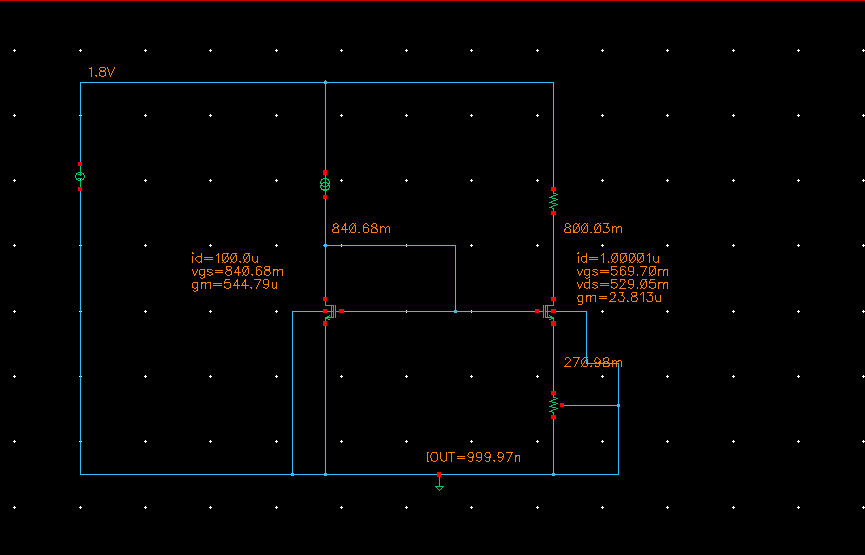
\includegraphics[width=\columnwidth]{fig_sch.png}
\caption{Cadence Virtuoso schematic with the DC operating point annotated.
$R_S$ is the 28-segment \texttt{resnsppoly} resistor
($r=\SI{270.98}{\kilo\ohm}$).}
\label{fig:sch}
\end{figure}

\section{Results and Discussion}

\subsection{Operating point}
At the selected resistance the simulator reports
$I_D(\mathrm{M2})=\SI{1.00001}{\micro\ampere}$,
$V_{GS2}=\SI{569.70}{\milli\volt}$, $V_{DS2}=\SI{529.05}{\milli\volt}$ and
$g_{m2}=\SI{23.81}{\micro\siemens}$; the source-node voltage is
\SI{270.98}{\milli\volt} and the current delivered to the load is
\SI{999.97}{\nano\ampere}. M1 operates in strong-inversion saturation
($V_{GS1}=\SI{840.68}{\milli\volt}$). Notably, the simulated $V_{TH}$ of M2
rises to \SI{612}{\milli\volt} through the body effect, so the output device
actually operates in moderate/weak inversion---exactly the regime where the
square-law hand model fails.

\subsection{Source-resistance sweep}
Fig.~\ref{fig:swrs} shows the simulated output current as $R_S$ varies from
\SI{150}{\kilo\ohm} to \SI{400}{\kilo\ohm}. The current falls monotonically
with increasing resistance, consistent with the source-degeneration
mechanism, and crosses the \SI{1}{\micro\ampere} target at
$R_S\approx\SI{271.0}{\kilo\ohm}$. Table~\ref{tab:iout} lists the output
current at selected resistances for cross-checking the curve.

\begin{figure}[!t]
\centering
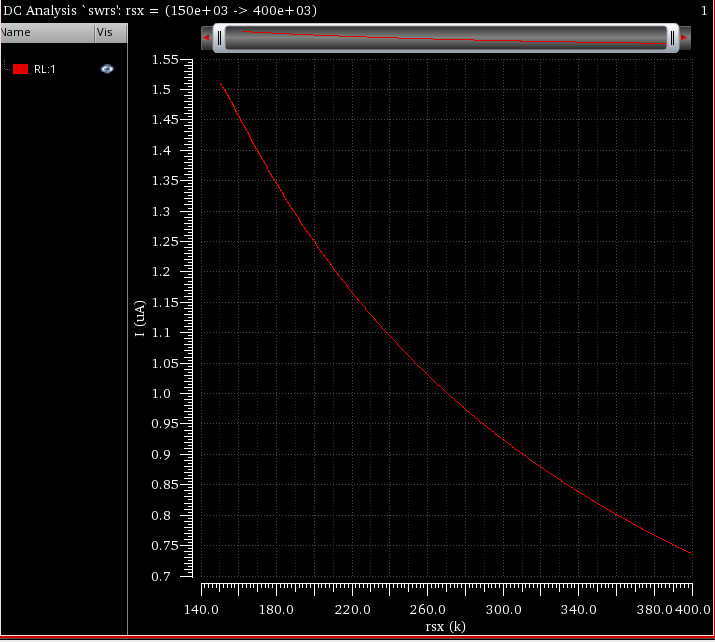
\includegraphics[width=\columnwidth]{fig_swrs.png}
\caption{DC sweep of output current versus source resistance (ViVA). The
\SI{1}{\micro\ampere} target is reached at $R_S\approx\SI{271.0}{\kilo\ohm}$.}
\label{fig:swrs}
\end{figure}

\begin{table}[!t]
\caption{Output Current at Selected Source Resistances}
\label{tab:iout}
\centering
\begin{tabular}{cc}
\toprule
$R_S$ (\si{\kilo\ohm}) & $I_\mathrm{OUT}$ (\si{\micro\ampere}) \\
\midrule
200 & 1.249171 \\
225 & 1.147868 \\
250 & 1.062244 \\
275 & 0.988911 \\
300 & 0.925380 \\
325 & 0.869789 \\
350 & 0.820722 \\
\bottomrule
\end{tabular}
\end{table}

The selected resistance is about 33\% greater than the \SI{204}{\kilo\ohm}
analytical estimate. The discrepancy reflects the difference between the
simplified hand model and the technology-model simulation---chiefly the body
effect and the moderate-inversion operation of M2. The drawn resistor (28
series segments of $\SI{24.195}{\micro\metre}\times\SI{1}{\micro\metre}$ at
\SI{400}{\ohm}/sq, total \SI{677.46}{\micro\metre},
\SI{270.98}{\kilo\ohm}) was centered by a separate sweep of the poly length,
which places the \SI{1}{\micro\ampere} point at
\SI{677.44}{\micro\metre}---within 0.003\% of the drawn value.

\subsection{Supply-voltage sweep}
Fig.~\ref{fig:swvdd} shows the DC response as the supply is swept from
\SI{0}{\volt} to \SI{1.8}{\volt}: the output current (upper trace) is
established once sufficient headroom exists, while the supply current (lower
trace) is dominated by the ${\approx}\SI{100}{\micro\ampere}$ reference
branch. The output branch requires adequate supply voltage before the
intended current is established.

\begin{figure}[!t]
\centering
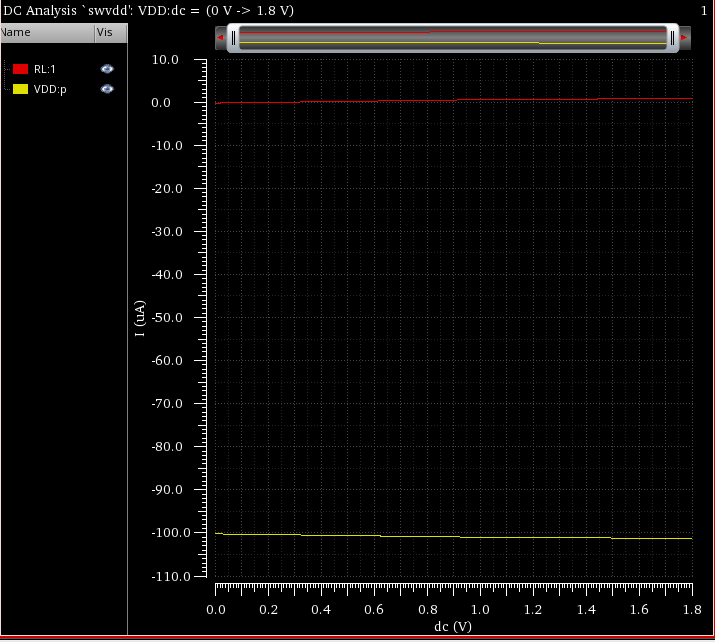
\includegraphics[width=\columnwidth]{fig_swvdd.png}
\caption{DC response during the supply-voltage sweep; upper trace is
$I_\mathrm{OUT}$, lower trace the supply-source current.}
\label{fig:swvdd}
\end{figure}

\subsection{Output compliance}
Replacing the load with a swept voltage source characterizes the mirror as a
current source (Fig.~\ref{fig:vout}). The output current saturates at
${\approx}\SI{0.9}{\micro\ampere}$ once $V_\mathrm{OUT}$ exceeds about
\SI{0.3}{\volt} and rises gently to \SI{1.18}{\micro\ampere} at
\SI{1.8}{\volt}, showing the finite output resistance of the simple Widlar
stage. For ${\pm}10\%$ current accuracy the output node must be held above
roughly \SI{0.3}{\volt}.

\begin{figure}[!t]
\centering
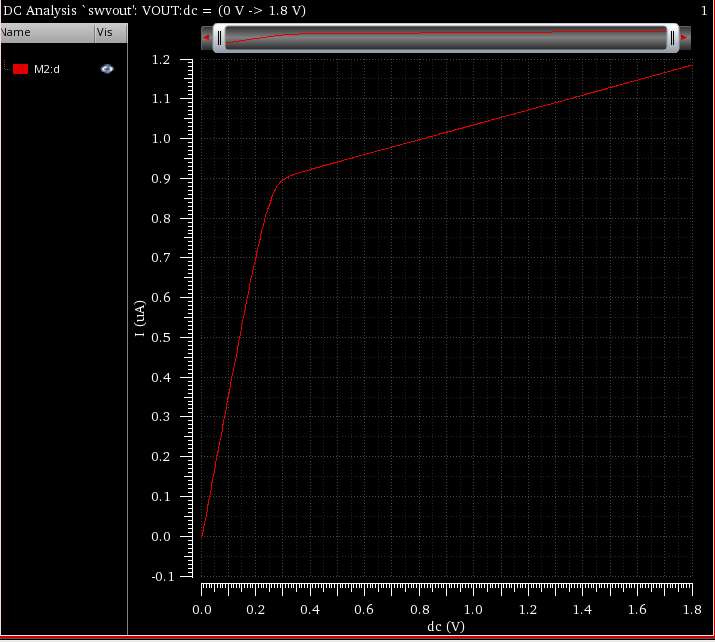
\includegraphics[width=\columnwidth]{fig_vout.png}
\caption{$I_D(\mathrm{M2})$ versus swept output voltage---output compliance
of the mirror.}
\label{fig:vout}
\end{figure}

\subsection{Transient behaviour}
A \SI{100}{\micro\second} transient at the operating point
(Fig.~\ref{fig:tran}) shows the output current steady at
\SI{999.9745}{\nano\ampere} with sub-\SI{5}{\pico\ampere} numerical ripple,
i.e.\ a stable DC current with no start-up anomaly in this configuration.

\begin{figure}[!t]
\centering
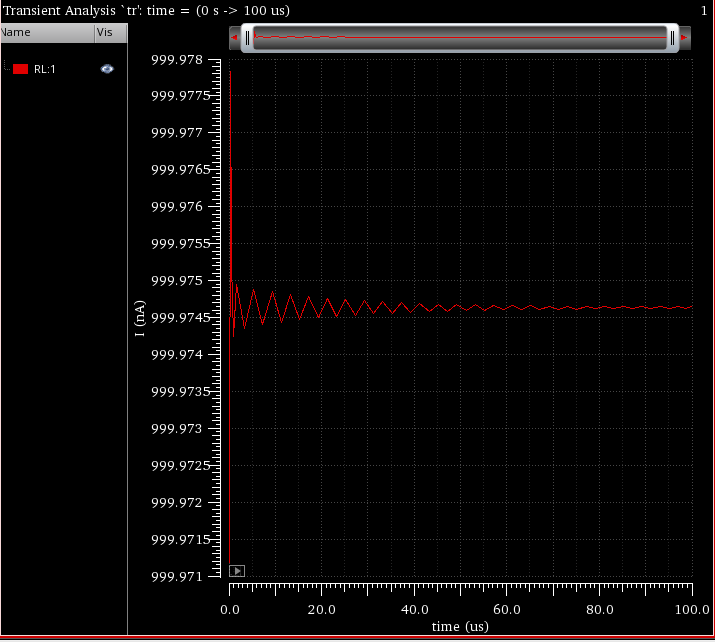
\includegraphics[width=\columnwidth]{fig_tran.png}
\caption{Transient response of the output current over
\SI{100}{\micro\second}.}
\label{fig:tran}
\end{figure}

\section{Layout and Physical Verification}
The mirror core (M1, M2, $R_S$) was laid out in Metal1 in a
${\approx}48\times\SI{37}{\micro\metre}$ area (Fig.~\ref{fig:layf}),
dominated as expected by the \SI{270.98}{\kilo\ohm} serpentine poly resistor.
M1 and M2 are single-finger \texttt{nmos2v} pcells with top gate straps
(Fig.~\ref{fig:laym}). M1 uses the pcell's integrated body tie---permissible
only because its source and bulk are both grounded, as the integrated tie
shorts S to B. M2, whose source sits \SI{271}{\milli\volt} above ground, uses
no local tap; its bulk is the common substrate, tied to ground by the taps of
M1 and of the resistor. The resistor carries its own substrate-tap strip,
required by the DRC substrate-stamping rule for its Psub region. The NS net
(M2 source to $R_S$) is routed down the right edge and enters the resistor's
PLUS terminal from below the pad row, keeping it clear of every ground shape.

\begin{figure}[!t]
\centering
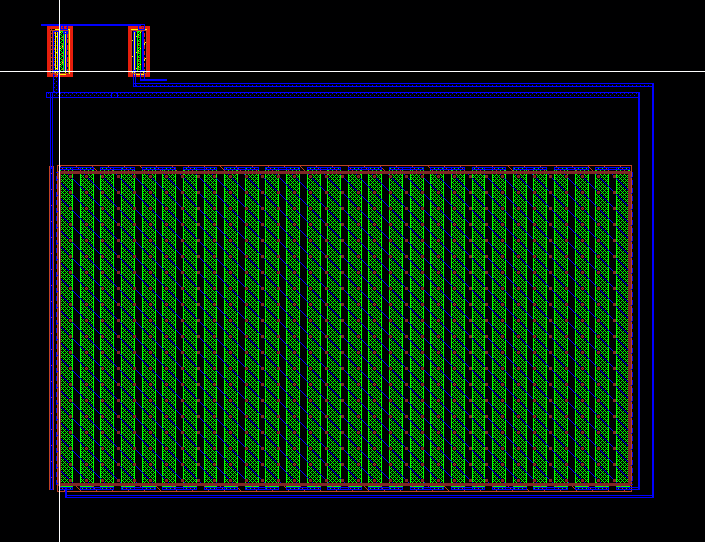
\includegraphics[width=\columnwidth]{fig_layf.png}
\caption{Complete layout: mirror pair (top left) above the 28-segment
serpentine \texttt{resnsppoly} resistor; common ground rail and right-edge NS
routing.}
\label{fig:layf}
\end{figure}

\begin{figure}[!t]
\centering
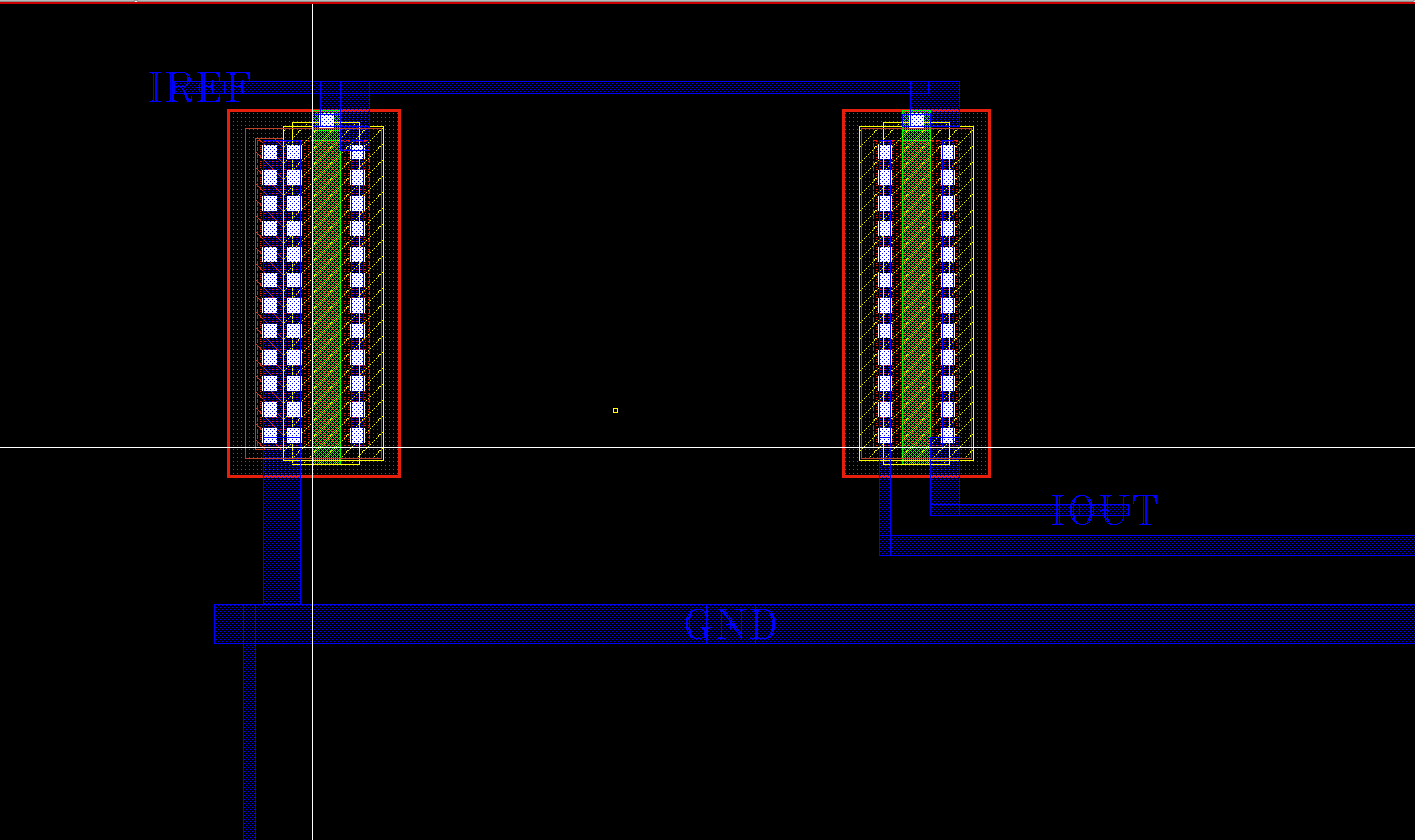
\includegraphics[width=\columnwidth]{fig_laym.png}
\caption{Detail of the transistor row: M1 (left, with integrated tap) and
M2, gate straps, and the IREF\,/\,IOUT\,/\,GND Metal1 routing.}
\label{fig:laym}
\end{figure}

Physical verification used the Diva decks shipped with GPDK090. DRC reports
zero errors. Layout extraction recognizes 2 \texttt{nmos2v} and 28
\texttt{resnsppoly} devices, all well formed. LVS compares the extracted view
against the schematic: the rule deck's series-resistor permutation merges the
28 drawn segments into the single \SI{677.46}{\micro\metre} schematic
resistor, and the netlists match with zero unmatched instances, nets or
terminals and zero size errors (Table~\ref{tab:pv}). The layout is therefore
electrically identical to the simulated circuit; at DC the residual layout
parasitic is ${\approx}\SI{87}{\ohm}$ of Metal1 trace resistance in series
with \SI{271}{\kilo\ohm}, a 0.03\% effect.

\begin{table}[!t]
\caption{Physical Verification Summary}
\label{tab:pv}
\centering
\begin{tabular}{ll}
\toprule
Check & Result \\
\midrule
Diva DRC & 0 errors \\
Extraction & 2 \texttt{nmos2v} + 28 \texttt{resnsppoly}, 0 errors \\
LVS devices & 30 vs 3 after series merge---matched \\
LVS verdict & ``The net-lists match'', 0 size errors \\
\bottomrule
\end{tabular}
\end{table}

\section{Advantages, Limitations, and Applications}
The source resistor provides a simple means of generating a small, stable
bias current without extreme device ratios, which is useful in low-current
biasing networks \cite{widlar,adi}. Its accuracy depends on the transistor
models, the resistor value and temperature coefficient, the available output
voltage, and device mismatch. The resistor dominates the silicon area---here
about 95\% of the cell---and consumes voltage headroom; the output current
departs from target when the output transistor lacks adequate drain voltage,
as quantified by the compliance sweep of Fig.~\ref{fig:vout}. Process
variation of the poly sheet resistance (${\pm}20\%$ across corners)
translates directly into output-current variation, a consideration absent
from ideal-resistor exercises.

\section{Conclusion}
An NMOS Widlar current mirror producing \SI{999.97}{\nano\ampere} from a
\SI{100}{\micro\ampere} reference at \SI{1.8}{\volt} was designed in Cadence
Virtuoso with the GPDK090 library. The square-law hand calculation gave
$R_S\approx\SI{204}{\kilo\ohm}$, while the technology-model sweep selected
\SI{271.0}{\kilo\ohm}---a 33\% correction dominated by body effect and
moderate-inversion operation of the output device. The resistor was realized
as an on-chip 28-segment poly serpentine, and the complete cell was carried
through layout, DRC (clean) and LVS (matched). The exercise demonstrates both
the value of analytical estimates refined by simulation with the intended
technology models, and the additional constraints---body ties, substrate
stamping, routing topology---that only appear at the physical-design stage.

\begin{thebibliography}{1}
\bibitem{widlar}
R.~J. Widlar, ``Low-Value Current Source for Integrated Circuits,'' U.S.
Patent 3,320,439, May 16, 1967. [Online]. Available:
\url{https://patents.google.com/patent/US3320439A/en}
\bibitem{adi}
Analog Devices, ``Chapter 11: The Current Mirror,'' Analog Devices Wiki,
section on the Widlar current source. [Online]. Available:
\url{https://wiki.analog.com/university/courses/electronics/text/chapter-11}
\bibitem{gray}
P.~R. Gray, P.~J. Hurst, S.~H. Lewis, and R.~G. Meyer, \emph{Analysis and
Design of Analog Integrated Circuits}, 5th~ed. Hoboken, NJ, USA: Wiley, 2009.
\end{thebibliography}

\end{document}
